\documentclass{beamer}
\usepackage{graphicx}
\usepackage{alltt}
\usepackage{tikz}
\usetikzlibrary{arrows}
\usetheme{AnnArbor}

\setbeamercolor{talktitle}{bg=green,fg=white}

\beamertemplatenavigationsymbolsempty
\title{A Survey of Sequence Assembly Methods}
\author{Martin D. Muggli}
%\institute{Computer Science Department, Colorado State University}
\date{September 4, 2015}
\begin{document}
\maketitle

\AtBeginSubsection[]
{
  \begin{frame}<beamer>
    \frametitle{}
    \tableofcontents[currentsection,currentsubsection]
  \end{frame}
}

\section{Background}
%\subsection{Shotgun Sequencing and de novo Assembly} % FIXME: make de novo emph and protected
%--------------------------------------------------------------
\begin{frame}
\frametitle{Shotgun Sequencing}

\includegraphics[width=\textwidth]{shotgun.jpg}

% http://cubocube.com/dashboard.php?a=344\&b=459\&c=1

\end{frame}
%--------------------------------------------------------------


%\subsection{Motivation}
%--------------------------------------------------------------
\begin{frame}
\frametitle{Motivation: Functional Element Proximity Relevance}

\includegraphics[width=\textwidth,height=0.8\textheight,keepaspectratio]{enhancer.png}

%https://en.wikipedia.org/wiki/Enhancer_(genetics)

\end{frame}



%\subsection{General Approach}
%--------------------------------------------------------------


\begin{frame}
\frametitle{Reconstruction: Overlap Graphs}
Overlap graphs require all-pairs alignment.  Classic method is O($n^2$).
\includegraphics[width=\textwidth,height=0.8\textheight,keepaspectratio]{olc.png}

%http://bmpvieira.github.io/assembly14/#/5
% modified from Schatz, 2010

\end{frame}
%--------------------------------------------------------------


\begin{frame}
\frametitle{Overlap: Sequence Alignment}
Optimal alignments are composed of optimal subalignments, giving rise to an O($n^2$) dynamic programming (DP) solution.
\includegraphics[width=\textwidth,height=0.7\textheight,keepaspectratio]{alignment.png}
%http://www.ibm.com/developerworks/library/j-seqalign/NWTab2.gif


\end{frame}




\section{Overlap Based de novo Assembly}

\subsection{DALIGN}
%--------------------------------------------------------------
\begin{frame}
\frametitle{Preferred Seed Matches in a DP matrix}
Most high scoring alignments will include runs of exact matches. Exact string matching then allows candidate pair identification.
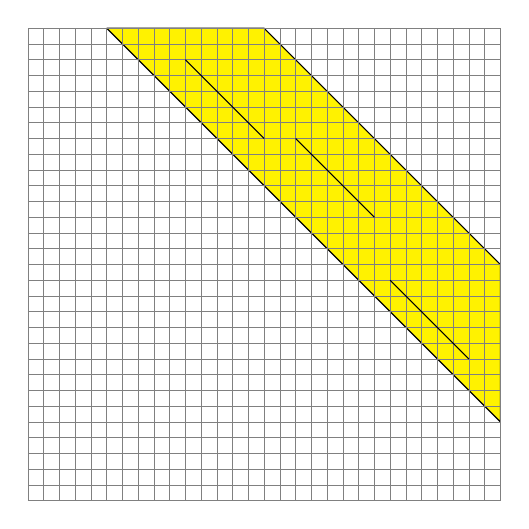
\begin{tikzpicture}[scale=0.2]
\draw[fill=yellow] (5,30) -- (15,30) -- (30,15) -- (30,5) -- (5,30);
\draw[help lines] (0,0) grid (30,30);
\draw (10,28) -- (15, 23);
\draw (17,23) -- (22, 18);
\draw (23,14) -- (28, 9);
\end{tikzpicture}

%\includegraphics[width=\textwidth,height=0.8\textheight,keepaspectratio]{fin.png}

% 
\end{frame}

%--------------------------------------------------------------
\begin{frame}
\frametitle{Non-Preferred Seed Matches in a DP Matrix}
Good seed matches should have conserved substrings between read pairs within a reasonable band.


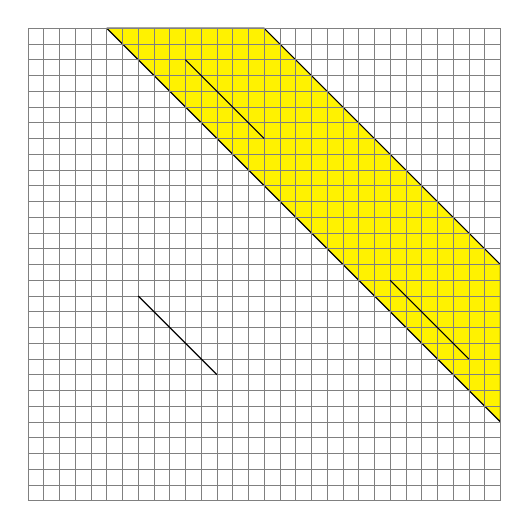
\begin{tikzpicture}[scale=0.2]
\draw[fill=yellow] (5,30) -- (15,30) -- (30,15) -- (30,5) -- (5,30);
\draw[help lines] (0,0) grid (30,30);
\draw (10,28) -- (15, 23);
\draw (7,13) -- (12, 8);
\draw (23,14) -- (28, 9);
\end{tikzpicture}

%\includegraphics[width=\textwidth,height=0.8\textheight,keepaspectratio]{fin.png}

% 
\end{frame}

%--------------------------------------------------------------
\begin{frame}
\frametitle{Non-Preferred Seed Matches in a DP Matrix}
Overlapping seed matches are a weak indicator of likely alignment.  
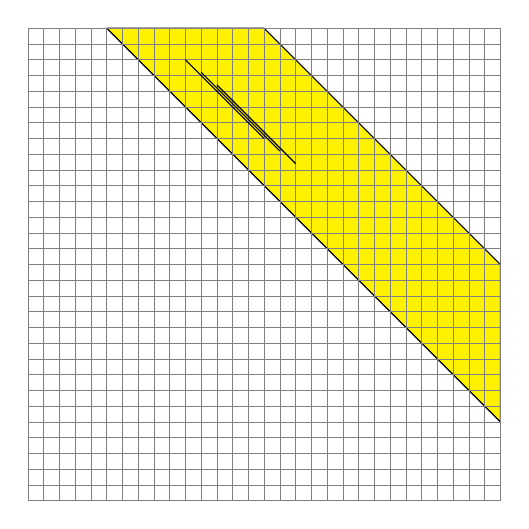
\begin{tikzpicture}[scale=0.2]
\draw[fill=yellow] (5,30) -- (15,30) -- (30,15) -- (30,5) -- (5,30);
\draw[help lines] (0,0) grid (30,30);
\draw (10,28) -- (15, 23);
\draw (11,27.2) -- (16, 22.2);
\draw (12,26.4) -- (17, 21.4);
%\draw (7,13) -- (12, 8);
%\draw (23,14) -- (28, 9);
\end{tikzpicture}

%\includegraphics[width=\textwidth,height=0.8\textheight,keepaspectratio]{fin.png}

% 
\end{frame}




%--------------------------------------------------------------
\begin{frame}
\frametitle{Bounded Seed Extension via Furthest Reaching Points}
Seeds can be extended by finding points within $D$ penalty reach of the start, growing for successive values of $D$.  Pruning allows expected O($n$).

\includegraphics[width=\textwidth,height=0.75\textheight,keepaspectratio]{furthestreaching.png}

% an O(ND) difference algorithm and its variations, myers
\end{frame}

%% %--------------------------------------------------------------
%% \begin{frame}
%% \frametitle{Burrows-Wheeler Transform}

%% \includegraphics[width=\textwidth,height=0.8\textheight,keepaspectratio]{bwt.png}

%% % 
%% \end{frame}

\subsection{String Graph Assembler}
%--------------------------------------------------------------
\begin{frame}
\frametitle{Burrows-Wheeler Transform}
Advantages:
\begin{itemize}
  \item Compresses repetitive strings well.
  \item \emph{Self index}: Encodes original string and can provide an index of the \emph{suffix array}.
\end{itemize}
\includegraphics[width=\textwidth,height=0.8\textheight,keepaspectratio]{bwt.png}

% 
\end{frame}

%--------------------------------------------------------------
\begin{frame}
\frametitle{SGA: FM-Index Backward Search for E.C. and Alignment}
Advantages:
\begin{itemize}
  \item Exact search in O($n$).
  \item Locate/count all matches concurrently.
  \item Encode edges with last column to first column mapping.
\end{itemize}


\includegraphics[width=\textwidth,height=0.8\textheight,keepaspectratio]{backwardsearch.png}


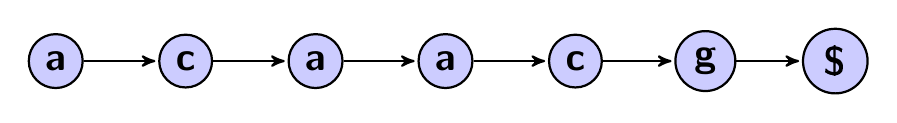
\begin{tikzpicture}[->,>=stealth',shorten >=1pt,auto,node distance=1.65cm,
  thick,main node/.style={circle,fill=blue!20,draw,font=\sffamily\Large\bfseries},scale=0.3]

  \node[main node] (1) {a};
  \node[main node] (2) [right of=1] {c};
  \node[main node] (3) [right of=2] {a};
  \node[main node] (4) [right of=3] {a};
  \node[main node] (5) [right of=4] {c};
  \node[main node] (6) [right of=5] {g};
  \node[main node] (7) [right of=6] {\$};

   \path[every node/.style={font=\sffamily\small}]
     (1) edge node [right] {} (2)
     (2) edge node [right] {} (3)
     (3) edge node [right] {} (4)
     (4) edge node [right] {} (5)
     (5) edge node [right] {} (6)
     (6) edge node [right] {} (7);
%     (7) edge node [bend angle=45] {} (1);

\end{tikzpicture}

% 
\end{frame}


\section{de Bruijn Graph Based de novo Assembly}
\subsection{de Bruijn Graph Background}
%--------------------------------------------------------------
\begin{frame}
\frametitle{de Bruijn Graph Assembly}
de Bruijn graphs have similar structure, but omit all pairs alignment.


\includegraphics[width=\textwidth,height=0.8\textheight,keepaspectratio]{debruijn.jpg}

% TODO: emphasize edge labels with k-mers



% http://genome.cshlp.org/content/20/9/1165.full
\end{frame}
%--------------------------------------------------------------

\begin{frame}[fragile]
\frametitle{$k$-mer Extraction}
\begin{verbatim}
ACCCAACCAC

ACCC
 CCCA
  CCAA
   CAAC
    AACC
     ACCA
      CCAC

\end{verbatim}
\end{frame}
%--------------------------------------------------------------

\begin{frame}
\frametitle{4-mer based de Bruijn Graph}
A de Bruijn graph can be constructed by:
\begin{enumerate}
\item Chopping reads into $k$-mers which become edges. Prefix and suffix ($k-1$)-mers become vertices.
\item Glue all all vertices with the same label.
\end{enumerate}

\includegraphics[width=\textwidth,height=0.7\textheight,keepaspectratio]{debruijn1.png}

% TODO: emphasize edge labels with k-mers
% http://gcat.davidson.edu/phast/img/debruijn/deBruijn1.png


% http://genome.cshlp.org/content/20/9/1165.full
\end{frame}
%--------------------------------------------------------------



\subsection{KMC 2}

\begin{frame}
\frametitle{$k$-mer Counting}

%\includegraphics[width=\textwidth,height=0.8\textheight,keepaspectratio]{}
\begin{alltt}
GCTAGCT

\end{alltt}

\begin{alltt}
\emph{GCTA}~ : 1 \\
\emph{CTA}~G : 1 \\
\emph{TA}~GC : 1 \\
\emph{A}~GCT : 1 \\
\end{alltt}

% 
\end{frame}



%--------------------------------------------------------------
\begin{frame}
\frametitle{Distributing $k$-mers}
Many consecutive $k$-mers have the same \emph{minimizer}, or lowest ranked $m$-mer substring.  The string covering all such $k$-mers is a \emph{super $k$-mer}. We can distribute super $k$-mers into bins, each associated with a fraction of possible minimizers.


\includegraphics[width=\textwidth,height=0.6\textheight,keepaspectratio]{MSPKmerCounter.png}

% http://www.cs.ucsb.edu/~yangli/MSPKmerCounter/index.html
\end{frame}



%--------------------------------------------------------------
\begin{frame}
\frametitle{KMC 2: ($k$,$x$)-mers}
Super $k$-mers and ($k,x$)-mers allow sharing of common $k$-mer substrings.

\includegraphics[width=\textwidth,height=0.8\textheight,keepaspectratio]{kx-mers.jpg}

% kmc2 paper
\end{frame}

\subsection{$k$-mer Genie}
%--------------------------------------------------------------
\begin{frame}
\frametitle{Challenge: Repeats}
Genomes contain repeated regions (red and green).

\includegraphics[width=\textwidth,height=0.8\textheight,keepaspectratio]{repeats.jpg}
% a-bruijn graph paper
% 
\end{frame}


%--------------------------------------------------------------
\begin{frame}
\frametitle{Challenge: Repeats}
Repeats longer than read data cannot be resolved in assembly, leaving tangled assembly graphs.  Assemblers can only emit the contiguous sequences spelled by non-branching paths.  These are \emph{contigs}.

\includegraphics[width=\textwidth,height=0.8\textheight,keepaspectratio]{debruijn_repeat.jpg}
% a-bruijn graph paper
% 
% TODO: sharpen
\end{frame}


%--------------------------------------------------------------
\begin{frame}
\frametitle{Challenge: Coverage}

Ideal read coverage would be uniform, allowing long $k$-mers to be glued between reads.

\begin{tikzpicture}
\node[align=left, above] at (5,10) {Genome};
\draw (0,10) -- (10,10);

\node[align=left, above] at (2,9.5) {Read 1};
\draw (0,9.5) -- (4,9.5);

\node[align=left, above] at (4,9) {Read 2};
\draw (2,9) -- (6,9);

\node[align=left, above] at (6,8.5) {Read 3};
\draw (4,8.5) -- (8,8.5);

\node[align=left, above] at (8,8) {Read 4};
\draw (6,8) -- (10,8);

\node[align=left, above] at (3,6) {$k$-mer};
\draw[|-|] (2,6) -- (4,6);

\draw[dotted] (2,6) -- (2,9.5);
\draw[dotted] (4,6) -- (4,9.5);

\end{tikzpicture}
%\includegraphics[width=\textwidth,height=0.8\textheight,keepaspectratio]{fin.png}

% 
\end{frame}

%--------------------------------------------------------------
\begin{frame}
\frametitle{Challenge: Coverage}

In practice, non-uniform coverage requires shorter $k$-mers, or else the assembly graph becomes disconnected.

\begin{tikzpicture}
\node[align=left, above] at (5,10) {Genome};
\draw (0,10) -- (10,10);

\node[align=left, above] at (2,9.5) {Read 1};
\draw (0,9.5) -- (4,9.5);

\node[align=left, above] at (5,9) {Read 2};
\draw (3,9) -- (7,9);

\node[align=left, above] at (7.5,8.5) {Read 3};
\draw (5.5,8.5) -- (9.5,8.5);

\node[align=left, above] at (8,8) {Read 4};
\draw (6,8) -- (10,8);

\node[align=left, above] at (3.5,6) {$k$-mer};
\draw[|-|] (3,6) -- (4,6);

\draw[dotted] (3,6) -- (3,9.5);
\draw[dotted] (4,6) -- (4,9.5);

\end{tikzpicture}
%\includegraphics[width=\textwidth,height=0.8\textheight,keepaspectratio]{fin.png}

% 
\end{frame}
%--------------------------------------------------------------
%% \begin{frame}[fragile]
%% \frametitle{$k$-mer Genie}
%% Innovations:
%% \begin{itemize}
%%   \item Sample the $k$-mer spectrum: \begin{verbatim}if hash(k-mer) == 0: counts.increment(k-mer) \end{verbatim}
%%   \item Choose $k$ with most distinct \emph{error free} $k$-mers.  Ideally, a distinct $k$-mer for every locus in the genome.
%%   \begin{itemize}
%%     \item Suboptimally small $k$-mers will collapse more repeats.
%%     \item Suboptimally large $k$-mers will mean genomic $k$-mers will not be covered by reads.
%%   \end{itemize}

%% \end{itemize}
%% %\includegraphics[width=\textwidth,height=0.8\textheight,keepaspectratio]{fin.png}

%% % 
%% \end{frame}

%--------------------------------------------------------------
\begin{frame}
\frametitle{Determining the Best $k$-mer Size}
\emph{Chikhi and Medvedev} show the $k$-mer size with the largest set of error free, distinct $k$-mers in a read set, revealed through \emph{abundance histograms}, predicts the best $k$ for assembly. 
\includegraphics[width=\textwidth,height=0.65\textheight,keepaspectratio]{kmer_abundance_regions.png}

% http://cristal.univ-lille.fr/~chikhi/pdf/2013-july-20-hitseq.pdf
\end{frame}

\subsection{Variable Order de Bruijn Graphs}

%--------------------------------------------------------------
\begin{frame}
\frametitle{Succinct de Bruijn Graphs}
Succinct de Bruijn Graphs represent edges as last-to-first mappings in the Burrows-Wheeler transform. Intervals denote nodes, and lower order views can be traversed by ``ignoring'' the least significant (leftmost) column.
\includegraphics[width=0.5\textwidth,height=0.7\textheight,keepaspectratio]{boss1.png}
\includegraphics[width=0.5\textwidth,height=0.7\textheight,keepaspectratio]{boss2.png}

% 
\end{frame}

\subsection{Paired de Bruijn Graph}
%--------------------------------------------------------------
\begin{frame}
\frametitle{Read Pairs}
Modern sequencing platforms read both ends of DNA fragments.
\includegraphics[width=\textwidth,height=0.8\textheight,keepaspectratio]{unpaired.png}

% 
\end{frame}


%--------------------------------------------------------------
\begin{frame}
\frametitle{Paired de Bruijn Graph}
Only gluing $k$-mers drawn from a left read when corresponding $k$-mers from the right pairs match detangles the graph.
\includegraphics[width=\textwidth,height=0.8\textheight,keepaspectratio]{paired.png}

% 
\end{frame}

\section{Reference Assisted Assembly}

\subsection{SOMA}
%--------------------------------------------------------------
\begin{frame}
\frametitle{Optical Mapping}
Optical maps give long range structure information.
\includegraphics[width=0.5\textwidth,height=0.8\textheight,keepaspectratio]{optical_map.png} 
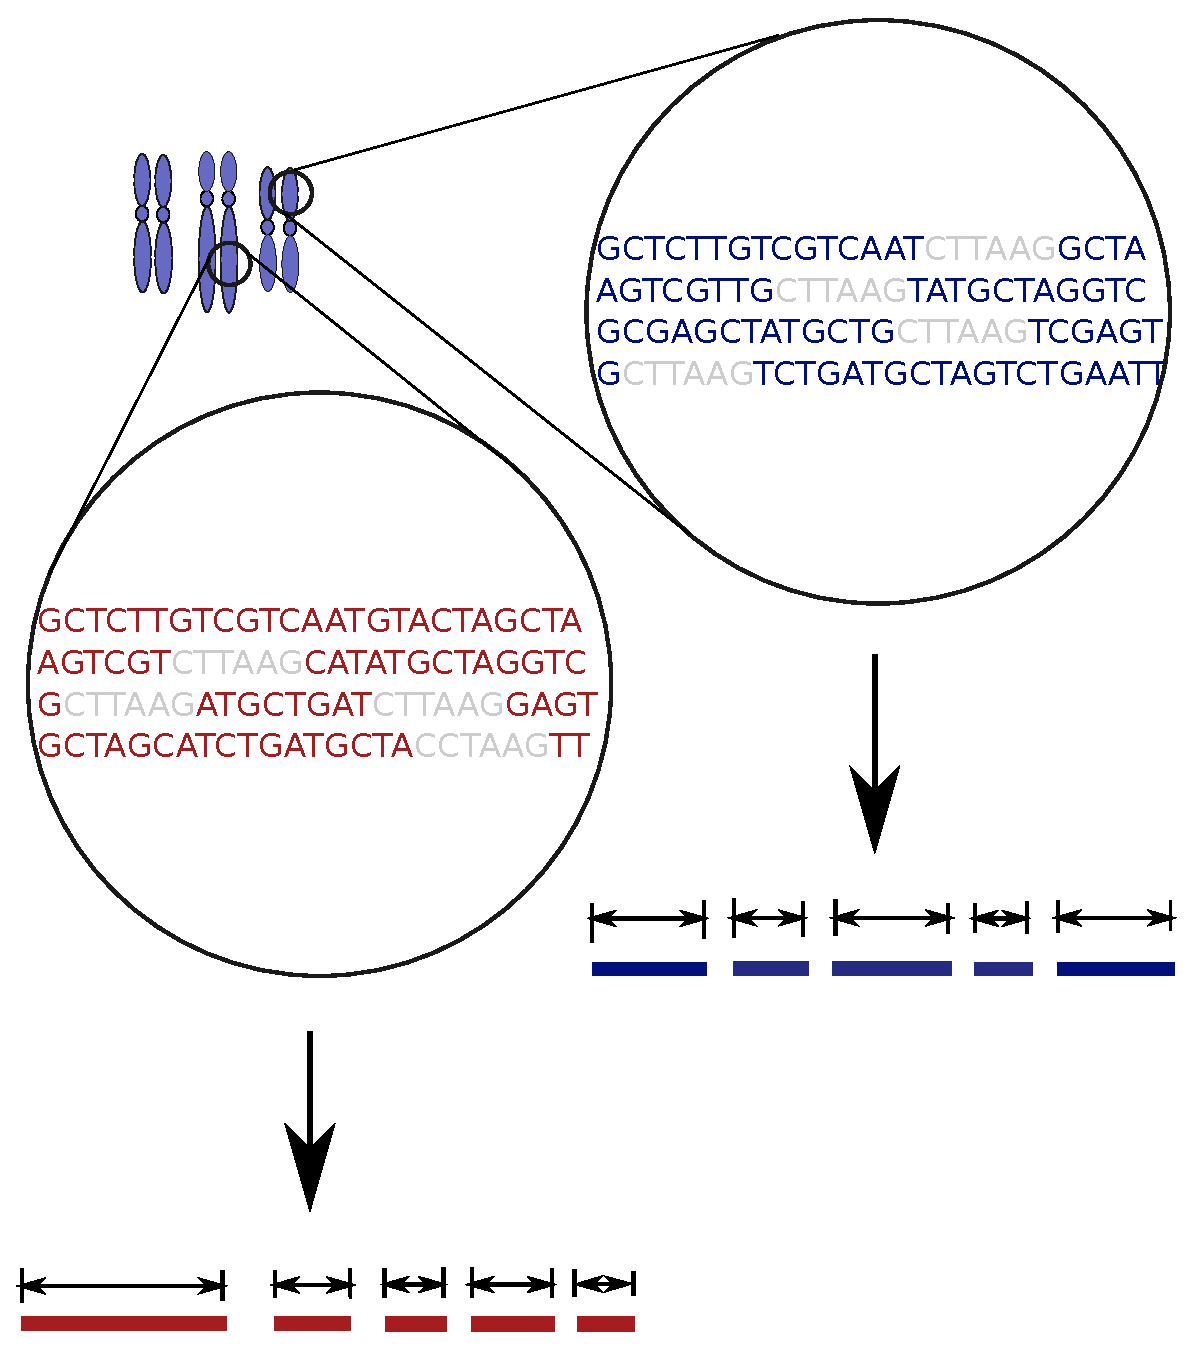
\includegraphics[width=0.5\textwidth,height=0.8\textheight,keepaspectratio]{ormpub.eps}



% 
\end{frame}
%--------------------------------------------------------------
\begin{frame}
\frametitle{SOMA}
SOMA can align contigs or scaffolds to a whole genome optical map for scaffolding and validation.
\includegraphics[width=\textwidth,height=0.8\textheight,keepaspectratio]{omalign.jpg}

% 
\end{frame}


\subsection{Reassembly and AGORA}
%--------------------------------------------------------------
\begin{frame}
\frametitle{Aligned References Guiding Graph Traversal}
%Long range structural information, either from optical maps (e.g. AGORA) or a reference genome (e.g. Parrish \emph{et al.}), can be aligned to edges in a de Bruijn graph.  This can guide traversal.   
\includegraphics[width=\textwidth,height=0.8\textheight,keepaspectratio]{reassembly1.jpg}

% 
\end{frame}
%--------------------------------------------------------------
%% \begin{frame}
%% \frametitle{Reassembly: Propagation and Pruning}

%% \includegraphics[width=\textwidth,height=0.8\textheight,keepaspectratio]{reassembly2.jpg}

%% % 
%% \end{frame}

%% \subsection{AGORA}
%% %--------------------------------------------------------------
%% \begin{frame}
%% \frametitle{AGORA}

%% AGORA is similar to read threading and reassembly.

%% %\includegraphics[width=\textwidth,height=0.8\textheight,keepaspectratio]{fin.png}

%% % 
%% \end{frame}





\subsection{GCSA}
%--------------------------------------------------------------
\begin{frame}[fragile]
\frametitle{Multiple Sequence Alignment As An Automaton}
A multiple alignment of a pan-genome can be represented as an automaton.

\begin{verbatim}
GACGTA-CTG
GACGTA---G
GATGTA-CTG
GAC-TACCTG
\end{verbatim}

%\includegraphics[width=\textwidth,height=0.4\textheight,keepaspectratio]{multalign.png} \\
\includegraphics[width=\textwidth,height=0.4\textheight,keepaspectratio]{automaton.png}
\end{frame}
%--------------------------------------------------------------
\begin{frame}
\frametitle{Prefix Range Sorted Automaton}
Prefix range sorting makes the prefix of all suffixes starting at a node distinct to that node.

\includegraphics[width=\textwidth,height=0.4\textheight,keepaspectratio]{automaton.png} \\
\includegraphics[width=\textwidth,height=0.4\textheight,keepaspectratio]{prefixrangesorted.png} 

\end{frame}
%--------------------------------------------------------------
\begin{frame}
\frametitle{Burrows-Wheeler Transform Of An Automaton}
In this form, backward search can be used for path matching.  Thus aligning reads or contigs against all known structural variants of a population.
\includegraphics[width=\textwidth,height=0.4\textheight,keepaspectratio]{prefixrangesorted.png} \\
\includegraphics[width=\textwidth,height=0.4\textheight,keepaspectratio]{automatonbwt.png} 

\end{frame}
\section{Extensions}
%--------------------------------------------------------------
\begin{frame}
\frametitle{Prune DALIGNs Work on Transitive Edges}

\includegraphics[width=\textwidth,height=0.8\textheight,keepaspectratio]{stringgraph.jpg}

% 
\end{frame}
%--------------------------------------------------------------
\begin{frame}
SGA showed their assembler used less memory but took significantly more time than de Bruijn graph assemblers.  As compressed suffix arrays have a variety of parameters, it would be interesting to see a runtime/memory tradeoff curve.

\end{frame}
%--------------------------------------------------------------
\begin{frame}
KMC 2 effectively uses shared structure to save both memory and time for the read data.  It would be interesting to see if shared structure could be immediately shared such as in a succint de Bruijn graph.

\end{frame}
%--------------------------------------------------------------
\begin{frame}
$k$-mer genie might be useful for picking the minimum overlap parameter for overlap based assemblers.  However, SGA notes that changing such parameters can be done much faster than de Bruijn graph assemblers.

\end{frame}
%--------------------------------------------------------------
\begin{frame}
The succinct de Bruijn graph effectively saves space and allows variable order traversal, however assemblers typically perform a graph simplification step and it's unclear how this structure can play a role in such an assembler as compressed structures are typically read only.

\end{frame}
%--------------------------------------------------------------
\begin{frame}
The paired de Bruijn graph only uses a $k$-mer from the right read to enhance support that two $k$-mers represent the same locus in the genome.  It seems plausible to use the rest of the bases in the paired end reads to further support or contradict this notion.

\end{frame}
 %--------------------------------------------------------------
\begin{frame}
AGORA only uses long non-branching paths in the de Bruijn graph for optical map alignment and only when unique.  This work might be extended to require all paths be in agreement with some not necessarily unique region of the optical map.

\end{frame}
%--------------------------------------------------------------
\begin{frame}
Using GCSA for pan-genome allows known combinations of structural variations without detecting new ones.  One might include a context free grammar of structural contituents and infer a grammar for the pan-genome.

\end{frame}
 
%--------------------------------------------------------------
\begin{frame}
Use both optical maps and reference genome for reassembly

\end{frame}
 %--------------------------------------------------------------
\begin{frame}
All methods here are content oblivious.

\end{frame}



\section{Conclusion}
\begin{frame}
\frametitle{Conclusion}
\begin{itemize}
\item Longer reads are better. 
\item More sources of data are better, especially if they are close to the donor’s genome. 
\item Data structures that capitalize on redundant data are useful. 
\item Partitioning problems into smaller independent problems are useful, either for reducing the memory high watermark or for parallelization (both of which favor large batches of independent work). 
\item Heuristics can be very effective in practice.
\end{itemize}
\end{frame}


%--------------------------------------------------------------
\begin{frame}
\frametitle{Acknowledgements}
I would like to thank the following people for reviewing my slides and presentation:
\begin{itemize}
  \item Darshan Washimkar
  \item Robert Raymond
  \item Thomas Harrison
  \item Yun Zou
\end{itemize}
\end{frame}

%--------------------------------------------------------------
\begin{frame}
\frametitle{}

\includegraphics[width=\textwidth,height=0.8\textheight,keepaspectratio]{fin.png}

% 
\end{frame}

%--------------------------------------------------------------
\begin{frame}
\frametitle{LF(): Last to First Mapping}

\includegraphics[width=\textwidth,height=0.8\textheight,keepaspectratio]{last2first.png}

% 
\end{frame}

%--------------------------------------------------------------
\begin{frame}
\frametitle{Minimizers}

\includegraphics[width=\textwidth,height=0.8\textheight,keepaspectratio]{minimizers.png}

%  robers 2004
\end{frame}

%--------------------------------------------------------------
\begin{frame}
\frametitle{Succinct de Bruijn Graphs: In Degree}

\includegraphics[width=0.5\textwidth,height=0.8\textheight,keepaspectratio]{bossin1.png}
\includegraphics[width=0.5\textwidth,height=0.8\textheight,keepaspectratio]{bossin2.png}


% 
\end{frame}

%--------------------------------------------------------------
\begin{frame}
\frametitle{Succinct de Bruijn Graphs: Out Degree}

\includegraphics[width=0.5\textwidth,height=0.8\textheight,keepaspectratio]{bossout1.png}
\includegraphics[width=0.5\textwidth,height=0.8\textheight,keepaspectratio]{bossout2.png}


% 
\end{frame}

%--------------------------------------------------------------
\begin{frame}
\frametitle{Determining \emph{error free} $k$-mers}

\includegraphics[width=\textwidth,height=0.8\textheight,keepaspectratio]{kmer_abundance_fit.png}

% http://cristal.univ-lille.fr/~chikhi/pdf/2013-july-20-hitseq.pdf
\end{frame}



\end{document}

% TODO:
% transitive edges

% FM-index?
% how contigs are made


% agora visual
% dalign sorting

% better de bruijn graph construction
% how read length matters for repeats

% succint de bruijn graph as a way to count k-mers

% order
%SGA
%dalign


%  depth of knowledge
% deep insight && critical analysis
% breadth of knowledge && acquire knowedge independently
% 

% chicken and egg problem: error correction and graph construction


%%%%%%%% darshun notes:
% center furthest reaching slide
% prune reassembly slides
% om + ref 
% preferred slide - more text
% k-mer redundancy needs bigger example
% new OM slide


%%%%%%% yun and rob feedback:
%% * takeaway per slide
%% * timeline/organization


%% problems/subproblems

%% 30 minute review
%% 5 summary
%% 10 opinion

%% missing definitions
%% too small figures

%% punchline

%% strings forshadow
%% section labels

%%%%% my org mode
%% * TODO review paper opinions/discussion
%% * TODO citations

%% * TODO transitive edges
%% * TODO acknowledgements slide





